\documentclass{sig-alternate-05-2015}

\RequirePackage[]{silence}
\WarningsOff[hyperref]
\usepackage {hyperref}

\begin{document}
% Copyright
\setcopyright{acmcopyright}

% DOI
\doi{10.475/123_4}

% ISBN
\isbn{123-4567-24-567/08/06}

%Conference
\conferenceinfo{WEA '16}{Copenhagen, 2016}

% --- Author Metadata here ---
\conferenceinfo{WOODSTOCK}{'97 El Paso, Texas USA}
% --- End of Author Metadata ---

\title{Bootstrapping a Software Ecosystem for Accelerating Second Language Acquisition}

% Alternative Titles
% (Growing a) Learning Software Ecosystem Based on Ubiquitous Monitoring and Adaptive Tutoring
% Lessons Learned while Growing a Learning Software Ecosystem
% How to Tame a Dragon - How to Grow an Ecosystem 
% A Platform for Growing a Learning Software Ecosystem
% Lessons Learned While Bootstrapping a Learning Software Ecossytem

\author{
Mircea F. Lungu \\
       \affaddr{SEARCH @ Johan Bernoulli Institute}\\
       \affaddr{University of Groningen}\\
       \affaddr{Netherlands}\\
       \email{i@mir.lu}
}

% \date{30 July 1999}

\maketitle

\begin{abstract}

Learning the vocabulary of a new language is a very slow and time consuming process which can take many years of dedicated study. 

In this paper I present the idea of an ecosystem which by monitoring the reading activities of a learner can build a model of their evolving knowledge and steer their future reading and studying sessions in such a way as to accelerate the speed with which they acquire new vocabulary. 

I describe a high-level architecture of the underlying platform dubbed Zeeguu, and exemplify some of the lessons learned while bootstrapping the ecosystem with several applications that complement each  other but are joined in the aim of accelerating vocabulary acquisition in a second language. 

\end{abstract}


\newcommand{\Lesson}[1]{ \vspace {0.3cm} \hrule \vspace{0.2cm} {\bf #1} \vspace{0.2cm} \hrule \vspace{0.3cm}}

\keywords{software ecosystems; software design; human-computer interaction; applied linguistics;}


%!TEX root=../main.tex

\section{Learning A New Language}

% it would be nice to talk about second language acquisition in the paper too if the term appears in the title

At any given moment millions of people are learning the vocabulary of a new language. The first steps in the acquisition of the new language are usually full of enthusiasm, but often the learner gives up once he realizes the magnitude of the task.

Indeed, once a learner has acquired the basic vocabulary of a foreign language, they are still many thousands of words away from actually mastering the new language. To improve their vocabulary they must constantly expose themselves to contexts in which the learned language is used at a level that is not too difficult but not too easy either -- that is, {\em they must study in the zone of proximal development}. Reading language textbooks is the traditional approach but more often than not textbooks being written for everybody are uninteresting for anyone.

Amazon has made a first step towards allowing the learner to read engaging texts by integrating translations and basic vocabulary exercises with their proprietary eBook reader device. Besides the limitations of being locked to a given dvice, this solution suffers also from the fact that the words being learned are locked in by Amazon. We will see later that this limits the possibilities of accelerating the speed with which vocabulary acquisition happens.

Another solution that the readers have is using Google Translate on the web. However, just as with Amazon, the translations that the user makes online are as of middle of 2016 not available outside the Google ecosystem. Thus the possibility of other applications benefiting from the knowledge of what the user is learning at the moment is also absent.

On the side of vocabulary rehearsal applications a plethora of solutions most of them being its own data silo. 


%!TEX root=../main.tex


\section {A Monitoring Ecosystem}

To address the disadvantages of the locked down nature of the existing infrastructures, we propose as a solution an open ecosystem that will combine their advantages while avoiding their limitations. The ecosystem should be built on the following principles:

\begin{itemize}

	\item The learners should be able to {\bf read anything that they find interesting}. Ubiquitous translations should be offered in context. 

	\item A user should have everywhere access to the words that he translated in the past and their context. Learning new words is much better done in context.

	% The context can be useful for further personalized exercises. To cover as many reading contexts as possible, it should be easy for new reading applications to join the ecosystem.

	\item An evolving model of the current state of the knowledge of the learner should be built by monitoring and observing as much as possible the users' interactions with foreign texts. The model should be available online for the applications members of the ecosystem.
	% The applications in the ecosystem that want to, should have access to this model.

	\item Intelligent agents should recommend reading and exercises that maximize the likelihood of encountering the most important learned words at the optimal times for every learner.

	\item The system should be open for any type of application that wants to contribute to it, either academic or industrial. The application would be able to make use of the information in the user profile as long as they contribute back to the ecosystem. 

\end{itemize}

We call this a {\em monitoring ecosystem} since the fact that the users activity is closely monitored is critical for the ecosystem. There can be different goals for monitoring ecosystems; in our case the goal is accelerating the learning process of factual information. 

The reasons for the various participants in this ecosystem are different, but everybody has something to gain: 

\begin{itemize}
	\item The Reader Applications. They receive information about the preferences of the user as well as his current knowledge of the various topics. They do not have to worry about storing the information about 

	\item The Trainer Applications. They receive information about the current knowledge of the user, and can better tailor exercises for them.
	
	\item The user. By using applications in the monitoring ecosystem, he has the confidence that his knowledge is mo

	\item The Core of the System. Can benefit from running anonymized analyses and discover trends and run scientific experiments.
\end{itemize}


%!TEX root=../main.tex


\section {The Zeeguu Ecosystem}
In this section we present a very high level architecture of a prototype of such an ubiquitous monitoring ecosystem as described in the previous section. It is built around a platform dubbed Zeeguu. Figure \ref{fig:architecture} presents a very simplified version of the Zeeguu platform and ecosystem.

\begin{figure}[h!]
	% \centering
	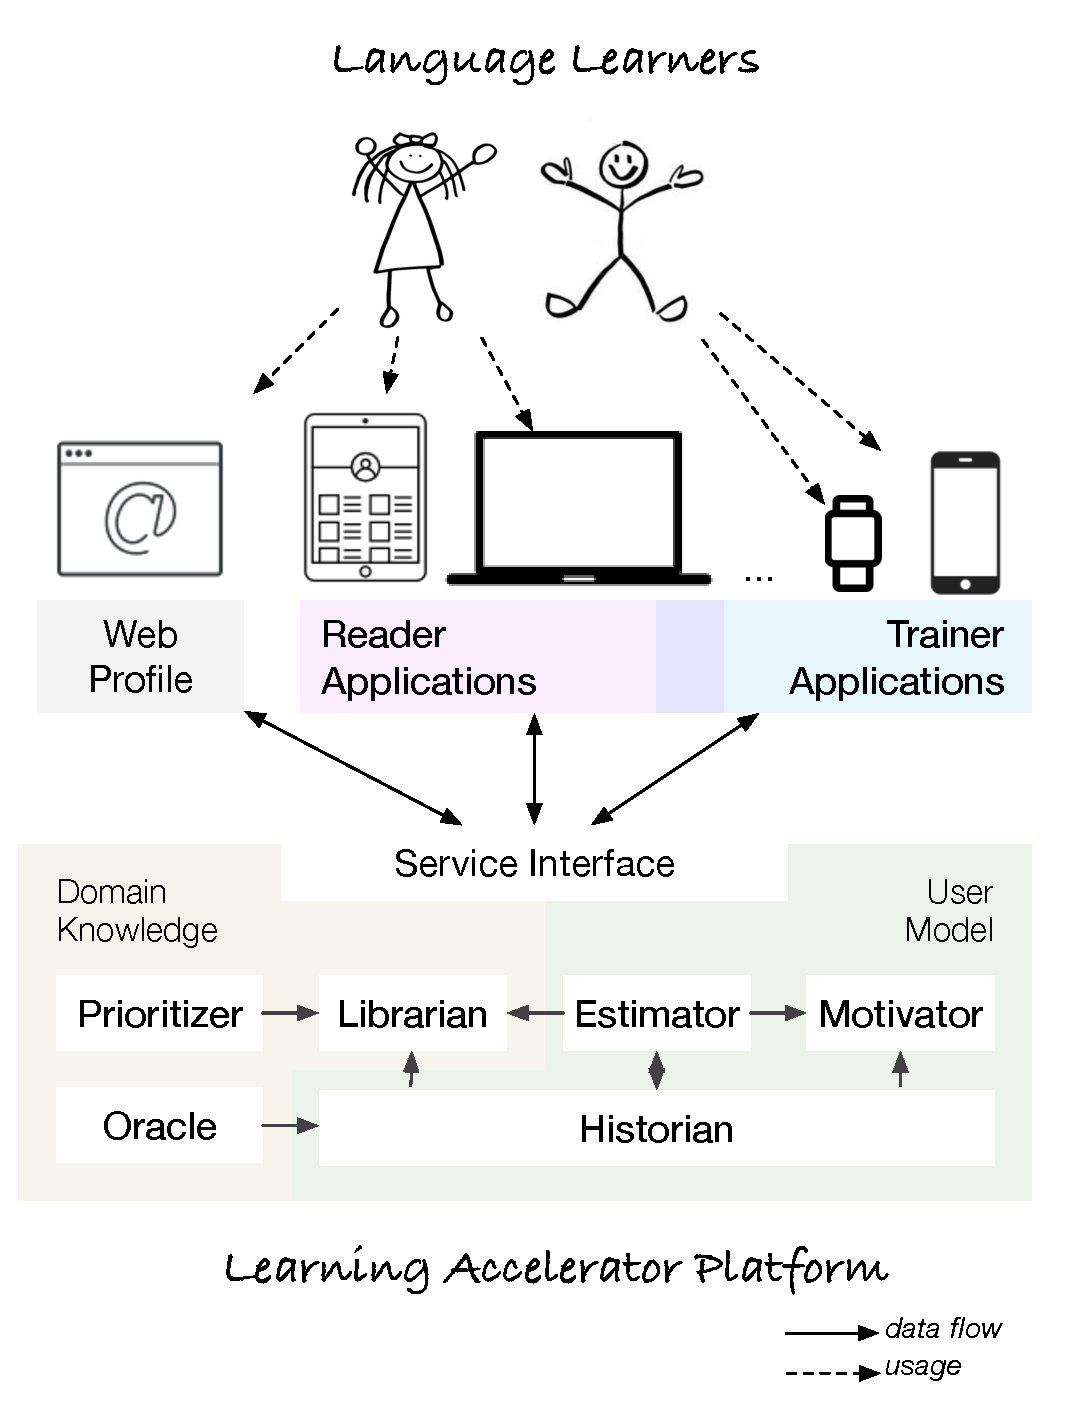
\includegraphics[width=0.98\linewidth]{images/zeeguu-architecture.pdf}
	\caption{A very high-level view of the architecture of the Zeeguu ecosystem}
	\label{fig:architecture}
\end{figure}

The figure presents only one type of actors, the language learners. The applicatoin developers are the ones who are building the main components with which the learners interact: 

\begin{itemize}
	
	\item {\bf Reader Applications} 
	support reading any kinds of materials in foreign languages. The reader applications must have two properties in common: 
		1) they should make it very convenient for the user to obtain translations for the texts he encounters in the foreign language. 
		2) they should report back to the server every event that provides a hint to the current user knowledge. In particular, every word that is being translated by the user indicates his lack of knowledge with respect to that particular word, and every word that is not being translate by the user indicates their knowledge of that word.
	
		\item {\bf Trainer Applications} support the learner in practicing the vocabulary and must interact with the user model. A trainer application can request from the user model store information on which words are to be learned by the learner. But a trainer application must also provide back to the central user model information about how well the learner behaves with respect to a given word, otherwise this information will be lost. 

\end{itemize}



The Zeeguu Platform is the core component of the learning ecosystem since it stores and orchestrates the exchange of information about the current and historical knowledge of the user. It needs to have several components, including: 

\newcommand {\archiblock}[1]{\item {\bf #1}}
\begin{itemize}

		\archiblock{The Translator} is a service which provides translations to the reader applications. It provides translations between many pairs of languages. It notifies the historian of every request it receives. 

		\archiblock{The Historian} is a data warehouse that sits at the core of a monitoring ecosystem. It records as much data as possible about all the interactions of a user with knowledge. 
		% all the interactions of a learner with texts in the foreign language that are mediated by the Reader applications.

		\archiblock{The Oracle} is a machine learning based agent that {\em estimates the current knowledge of the learner} based on the information received from the Historian. It decides what are the most likely items that must be studied by the learner. 


		\archiblock {The Librarian} is a web crawler that uses natural language processing techniques together with the information from the Oracle to support its goal of {\em providing recommendations to the learners} about which materials to study which are at the appropriate difficulty level as well as interesting enough for the learner.

		\archiblock {The Motivator} is an agent that uses gamification techniques to keep the learner motivated. It uses information from the Historian to be able to report on a learners engagement. It uses information from the Oracle to be able to provide feedback on the actual learning progress. 

\end{itemize}

Note that as the Figure \ref{fig:architecture} suggests, the Reader Assistants and Trainer Agents need not be disjoint applications, but one application could provide both.

It might appear intuitive for the reader that the more contexts in which the reader is supported by applications from the ecosystem, the better the knowledge model of that learner that can be built, and the better the user experience. Such a learning ecosystem can thus present a network effect where its value will increase more than linear with the number of applications that contribute to it.

% Somewhere, we still have to discuss the question of: 
% - How are we going to maintain this ecosystem? who will provide the data storage and translation facilities for the long run? 
% - What are the incentives for new players to join the ecosystem?
% - ... 



%!TEX root=../main.tex


\section {Bootstrapping the Ecosystem}

In order to obtain a {\em minimal viable ecosystem} several of its key components must be in place. This section presents in a quasi chronological order several milestones in the evolution of the  ecosystem over the recent years. 

In each of the subsections, we take the chance to step back and highlight one or several open questions that we think might be faced by future builders of such monitoring ecosystems. 

\subsection {A Minimal Viable Ecosystem}
The first milestone was releasing four main components of the ecosystem: 

\begin{itemize}
	\item One {\em reader application} implemented as a Chrome extension. It allows a learner to read any text and obtain in-place translations on any website as long as it is visited within the Chrome Browser\footnote{Available at: \url{https://zeeguu.unibe.ch/chrome}}. 

	\item An initial version of the Zeeguu platform, containing the Historian, a Translator that relies on external services, and a very basic version of the Oracle, exposed via a REST API. \cite{Lung16zeeguu}. 

	\item A basic {\em Web Profile} application\footnote{The web application is available at \url{https://zeeguu.unibe.ch}} that provides account management, and a simple interface to present the reading history of a learner. 

	\item One very simple {\em trainer application} which asks the learner to recognize a given word within its context. The words and contexts are selected from the past readings of the learner.

\end{itemize}

The web application and the REST API were deployed together on the same server as Python-based applications and the separation between them was not well enforced. This came to hunt us later when we discovered that as we were extending the REST API for other applications, we were duplicating functionality already existent in the web profile application. Surely a little technical debt can speed up the initial bootstrapping phase, but we think that it would have been better to treat internal applications as future third-party applications already from the begining.  
% They represent a test case for functionality, and in the long run this will avoid duplicated code.
}

The Chrome extension as a reader application posed two main limitations: 
	1) not everybody is reading his foreign language texts on their computer and,
	2) some users are circumspect when it comes to installing third-party browser extensions. 
In truth, this circumspection is well founded since a browser extension has access to all the information on the pages the user visits. 

In our case, we made our extension be active only on those pages where the user explicitly activates it. However, the only way a user can be completely confident that no information is leaking is reading the code. And although the code is open-source, this is not a realistic request from a language learner. A first question about privacy in a monitoring ecosystem emerges: 

\Question {Can a monitoring ecosystem ensure and prove to its users that individual applications do not have access to more data than they are allowed to?}
% TODO: could ask a question about -- how do you prove that a chrome extension does not track more data than it is supposed to?


\subsection {Adding a Reader for Android}

The Zeeguu Reader for Android was implemented as a bachelor project by Schwab \cite{Schw16thesis}. The application is written in Java and functions as an RSS feed reader. The architecture of the application makes a clear distinction between: 

\begin{enumerate}
	\item The {\em Zeeguu Android Library}\footnote{\url{https://github.com/linusschwab/zeeguu-android-library}} which eases the communication with the REST API and is released as a separate open-source component, and 
	\item The actual reader application which focuses on the usability of offering textual translations in context
\end{enumerate}

The separation has proven to be a good choice since a second Android application -- a Dictionary implemented by Giehl \cite{Gieh15a} could readily benefit from the API component.

During usability studies, however, we learned that a subset of the test users found it inconvenient to have both the Reader and the Dictionary applications installed. They would have preferred a single application. This raises another open question:

\Question {When is it better to fuse multiple applications into a single one?}

One of the features of the Android Reader application was ranking news items based on their difficulty with respect to the current estimated knowledge of the learner. Since such an algorithm would very likely be required for other applications in the ecosystem, we decided to move this functionality in a separate component on the server (the Librarian) and expose it using an API. 

The Android Reader relies on Feedly, a third party API, to track news feeds. This turned out to be very cumbersome for learners since they required to create a new account to a different service, before using the application. This problem was solved in the case of the iOS reader.

\subsection {Adding a Reader for iOS}


Oosterhof \cite{Oost16reading} implemented a reader for iOS. The application written natively in Swift eliminates the explicit dependence on third party services like Feedly. Instead the burden of extracting feed information from pages and monitoring a users preferred feeds has been moved into a separate agent inside of the platform. We discussed earlier how the Librarian was also migrated to the platform from an app. This illustrates our assumption that having all the information about a learner stored in a single central place simplifies data processing and user modeling. However, a more distributed design cold also be investigated.

% \Question {Do learner modeling components tend to migrate towards the platform in a monitoring ecosystem?}

% Correspondingly the REST API grew with new functionality.

The architecture of the iOS application made again a clear separation between a component which was to interact with the API\footnote{\url{https://github.com/mircealungu/zeeguu-ios-library}} and the actual GUI of the application. Since for every new language the developer must handwrite a new API interface to  communicate with the core services, we ask: 
 % one question is raised:
% . This made us realize the missed opportunity of automatically generating the APIs for different languages. However, as far as we are aware, no such generator exists for the Python technology stack used. 

\Question {Would the use of technologies that enable the automatic generation of APIs increase the adoption by lowering the barrrier of entry to the ecosystem?}


\subsection {Adding a Smartwatch Trainer}

According to current estimates, the wearable market\footnote{Which includes fitness trackers and smartwatches, so the number of smartwatches is likely smaller} will pass 111 million shipped devices in 2016, up from 80 million shipped in 2015. 

The ease with which a user can consult his smartwatch makes it an interesting platform for a learning strategy called {\em micro-learning} known for quickly closing skill and knowledge gaps  \cite{Dear12}. Having a trainer on the smartwatch would make it easy for the learner to take advantage of and study during dead moments of the day (e.g. waiting for the barista to prepare a cappuccino).

A trainer, dubbed {\em Time to Learn}, was implemented for the Gear S2 smartwatch by Haan and Nienhuis\cite{Nien16time}. The Gear S2 device runs on the Tizen mobile operating system and applications for it are written using HTML5 and Javascript.

To support micro-learning, the information on the smartwatch should be readily available when a learner looks at the watch. Thus, Time to Learn is implemented as a watch face which is divided in two: the top half presents the usual watch information, while the bottom part represents a word recognition challenge for the learner. The word to be displayed is selected based on an Oracle recommendation. 

After every challenge, the learner provides feedback on whether he knew a given word or not. This feedback is sent back to the Historian so it can be used in the future by the Oracle.


On the platform, the Oracle has to take into account the existence of the smartwatch events explicitly and treat them in a different way than the events from the web based trainer. 
% This forces the Oracle to be aware of the individual applications in the ecosystem, or at least of some of them -- in our case, the trainer applications. 
Theoretically, the Oracle could be implemented with machine learning technologies, in such a way as to be agnostic about the existence of the indiviudal trainers. However, this direction needs to be explored further.

\Question {Is it possible to let new applications join a monitoring ecosystem without having a central component that is aware of the existence of the individual applications?} 



%!TEX root=../main.tex

\section {Reflections}

It is still not clear when and if this ecosystem will 
take on a life on its own. Until now, all the 
applications that were added, have been in one way
or another supported by the creator. The challenge
of incentivizing external application developers and
defining policies that will benefit all the 
players still remains \cite{Jans09agenda}. 


Also, this is not the first ecosystem that aims to track 
the interactions of a user with data and build a better 
user model based on this; many commercial companies do it too. 
However, the goals of these companies are usually economic, 
while the goal of our ecosystem would be research and education.

It would seem thus, that since profit is not the main
goal of such an ecosystem, we should be confronting
with different problems than those enterprises where 
profit is critical. However, the economical 
sustainability of the platform when hosted in academia
is still an open question. The hosting costs of the 
core components are at the moment not significant 
but they could become large in the eventualily of 
a massive growth.


One way to do this would be to unequivocally show 
the benefits it brings to the learners. Based on 
early user studies and the feedback we received 
from individual applications we can say that such
an ecosystem shows promise. But more work has to 
be done for this. 

% One other aspect that has not been discussed here
% but which will have to be dealt with at some point 
% is the privacy issue. How can we make sure that 
% private information about a reader does not leak
% between applications. 

% Finally, there is no claim or expectation that the 
% lessons derived here hold beyond the given case study. It 
% might be and it is our hope that they can be of 
% use for other learning ecosystem development
% projects, but until more such results 
% are published, this remains to be seen.



% - how to insure privacy? should everything in the profile be visible for all the apps?


%!TEX root=../main.tex

\section{Conclusion}

The paper presents a proposed architecture and reports
several lessons learned while bootstrapping an ecosystem designed for accelerating vocabulary acquisition.
The paper also lists several open research questions which are probably relevant for other types of monitoring ecosystems. 

% a platform that
% aims to support learning software ecosystem. 
% but probably such an approach can be extended to other types of learning. 



\vspace{0.5cm} 
\noindent {\bf Acknowledgements} The author would like to thank
Jens Knodel and Anca Lungu for feedback on early versions 
of this paper. 

\newpage

\bibliographystyle{IEEEtran}
\bibliography{mir-biblio/aslan,mir-biblio/eco}



\end{document}
